\chapter{Validation}
\section{implémentation}
expliquer comment on a fait pour implémenter. Quel était les moyen mis en place pour faire un bon logiciel.

schéma uml

comcomber

rspec

factories

metrics (travis, gemnasium, codeclimate, coveralls, railsbestpractice)

\section{Expériences}
Cette section aborde les expérience réalisé pour ce travail. Ceci commence par une après midi chez kidscode, vient ensuite le printemps des sciences pendant lequel environ 80 élèves ont tester l'application. Enfin, vient une analyse des experience a travers des formulaire remplis par les élèves et les professeurs. %TODO pourquoi et comment
\subsection{kidscode}
\label{kidscode}
Dans le cadre de ce mémoire plusieurs expérience ont été menée. La première s'est déroulé chez Kidscode. Cette organisation a été présenté dans la section \ref{init-kidscode}. C'est une petit initiative locale qui apprend la programmation à 10 enfants âgé de 10 a 14 ans.

\subsubsection{Contexte}
\label{context-kidscode}
Il est important de définir le contexte et le publique de l'expérience car il peut avoir une influence considérable sur l'analyse des retours.\\

Lors de cette expérience le publique était un publique de 10 enfant de 10 à 14 ans ayant déjà fait une demi année de programmation dans le cadre du projet Kidscode. Le niveau de c'est enfant n'est donc pas à négligé. Ils étaient déjà habituer a compiler un programme et maîtrisaient les principaux concepts de la programmation.\\

\subsubsection{Buts}
Le but poursuivit dans cette expérience est de validé l'utilisabilité de la plateforme et également le niveau de difficulté des missions proposées. Un autre but était également de se familiariser avec le public et en petit groupe pour pouvoir pour la seconde expérience gérer un groupe plus conséquent et moins discipliner.

Ce dernier point pourrait semblé ne pas être justifier dans le cadre d'un mémoire universitaire, mais la manière d'aborder les enfants et probablement aussi important de la qualité de l'application. Pour limiter le plus possible les biais dû a un manque de pédagogie ou d'expérience dans la gestion d'un groupe d'enfant, il était important de pouvoir avoir cette première expérience.
\subsubsection{Déroulement}
L'expérience s'est déroulée pendant un peu plus d'une heure. Les enfants avaient les premières heures l'activité kidscode normalement et la dernière heure était dédier à l'expérience. 

Comme le changement d'activité était clairement marqué, le début de l'expérience fut marqué par beaucoup de perte d'attention et de dissipation. Un fois le groupe repris en main, les jeunes ont directement montré un intérêt très marqué. D'une part pour l'interface qu'ils découvraient et qui semblait leur plaire. D'autre part pour une compétition qui s'est très vite mise en place au seins du groupe.\\

Comme expliqué dans la partie précédente \ref{context-kidscode}, le public avait déjà de bonne notion de programmation par rapport au publique visé par ce mémoire. Les première missions sont donc passées très vite. Les seuls points de ralentissement étaient principalement des problèmes de lecture des consignes. 

A ce moment, les consignes étaient toutes écrites. Cela a posé un problème car les jeunes ne prenaient pas le temps de les lire et donc ne savaient pas quoi faire une fois dans les missions. Ceci malgré la possibilité de retrouver les consigne via les menu de l'application. Ce manque d'intérêt pour les consignes ne venait pas d'un problème de niveau de lecture mais simplement d'une impatience face a l'expérience et donc au manque de rigueur dû à leur âge.\\

La compétition que les jeunes ont mis en place dès le début a eu un effet bénéfique pour leur évolution car elle leur donnaient la motivation de réaliser les défit proposé. Ceci était fort marqué à chaque passage de mission. Chaque fois qu'un groupe finissait une mission il était important pour eux de le signalé et cela leur donnait une satisfaction qui les poussait réaliser la mission suivante.\\ %d'ou le fait que plein de petite mission est approprier.

Dans les délais imparti, tous sont arrivé à la mission final du chien et du chat \ref{chien-chat}, mais personne n'a réussi à la finir. Quand a sonné la fin de l'expérience, beaucoup nous ont demander comment faire pour montrer ce qu'ils avaient réaliser à leur famille et comment faire pour continuer leurs réalisations.

\subsubsection{Analyse}
\label{analyse-kidscode}
L'expérience c'est dans l'ensemble très bien déroulé et les participants ont beaucoup apprécier.

Certaines amélioration ont été apporté à l'application dû à cette expérience. C'est ces modification qui seront discutée maintenant.

\paragraph{Changement dans les missions}
Une mission, \texttt{répète et répépète} a été retirer car elle s'est avéré peu intéressante en concept et peu accrocheur pour les enfants. Cette mission avait pour but de faire découvrir les fonctions d'affichage de texte. Un personnage devait répéter ce que disait un autre. Pendant cette mission, beaucoup d'enfants se sont dispersé parce qu'ils s'embêtaient et que ce n'était pas assez concret. Cette mission a été remplacé par \texttt{Soyons courtois} décrite en section \ref{mission-courtois}. Cette nouvelle mission est beaucoup plus dynamique que la précédente, permet à l'étudiant de se déplacer et utilise les capteurs de collision introduit dans la mission précédente.

\paragraph{Ajout d'un bouton "resset"}
Lors de l'expérience un groupe d'enfants a réussi suite a une série obscure d'opération à casser l'environnement de la mission. Pour palier à ce genre de problème, un bouton "resset" a été rajouter dans l'interface de Snap! pour pouvoir réinitialiser la mission courant à celle de départ.

\paragraph{Ajout de vidéo d'introduction}
Comme observé dans cette expérience, les jeunes ont tendance a ne pas lire les textes explicatifs des missions. Ceci résulte qu'ils ne savent pas quoi faire dans la mission et donc ne fond pas grand chose de productif. Des vidéos d'introduction on donc été rajouté au début de chaque mission juste au dessus de l'explication de la mission. Cette vidéo explique le but de la mission et les instructions pour y arriver. Comme cela les étudiants regarde une fois la vidéo 

% mission supprimer du a kidscode + bouton resset
% les viédo youtube
% nouveau bouton dans l'interface du a kidscode

\subsection{Printemps des sciences}
Cette expérience s'est dérouler dans le cadre de la semaine science infuse. Lors de cette dernière des écoles, du primaire et du secondaire, viennent participer à des animations dans les universités. C'est lors de cette semaine science infuse que l'expérience s'est passée avec quatre groupes d'enfants de différent âge et horizon. Ces activité durait au total une heure trente minute avec les temps d'installation et de prise en charge. Lors de toute ces expériences les élèves était en paire programming et donc a deux devant un ordinateur.

\subsubsection{Contexte}
Le but de cette expérience dans le cadre de sciences infuse était de valider l'application sur un grand nombre d'enfants d'horizon et d'âge différent. Lors de cette expérience, 74 étudiants âgé de 11 a 13 ans. Les enfants étaient réparti en 4 classes, deux de sixième primaire et deux de première humanité.

L'origine des jeunes est également varié. Il y avait des classe de Chimay de Bousval et de Ottignies. Ceci était souhaité pour avoir un échantillon plus représentatif de la population.

\subsubsection{Buts}
Le but principal de cette expérience était de confronter l'application à sont usage réel dans des classe d'étudiants. De pouvoir observer comment cela se déroule en réalité et ressortir une analyse des besoins spécifique qui manqueraient à l'application.

Un autre but poursuivit était l'évaluation de l'âge idéal et du niveau de difficulté des missions pour des néophytes. En effet, lors de l'expérience précédente, le publique était volontaire et avec déjà un background en programmation. De par ce fait, le niveau des missions s'était avéré un petit peu faible.

Un dernier but était évidement de récolter l'avis des personnes concernées, à savoir les étudiants, sur l'application. Observer leur réactions et leur intérêt ou non pour la solution proposée.

\subsubsection{Déroulement}
\paragraph{École sainte Marie} La première classe à avoir tester ma solution est celle de sixième primaire de l'école sainte Marie à Bousval. Le groupe était composer d'une petite vingtaine d'élèves.

L'activité s'est déroulé avec une petite contrariété informatique. En effet le moteur JavaScript des machines mises à disposition était très lent. Ceci n'a pas compromis le déroulement de l'activité mais fut à parfois moment une source de frustation pour certain élèves très enthousiaste.

Lors de la mise en place une petite démonstration de l'interface a été présenté pour les familiariser à Snap!. Suite a cela les élèves ont été invité à créé un compte par ordinateur. La démonstration s'arrêtait à la première vidéo de la première mission.\\

Une fois la première vidéo passée, les élèves ont directement entamer la première mission. Une crainte était que grâce au lecteur \texttt{youtube} il regarde d'autre vidéo, mais il n'en fut rien et leur curiosité était assez forte pour les garder dans l'application.

La première mission était celle de la voiture qui est décrite à la section \ref{mission-voiture}. Un des concepts difficile aborder dans cette mission est la structuration mentale de leur script. C'est effectivement ce qui fût le plus difficile avec cette classe. La voiture revenait à son point de départ à chaque lancement du script. Mais globalement après quelque essaies-erreurs, ils ont tous réussi rapidement la mission.\\

Une fois la première mission fini, il a été nécessaire de leur rappeler comment sauvé et revenir à la liste des missions. Mais les fois suivante, entre la mission deux et trois, comme entre trois et quatre, les jeunes n'ont plus demander comment il fallait faire. Leur seul crainte était de savoir si leur mission avait bien été enregistrer sur le serveur.\\

A la fin du temps imparti, tous les élèves avait atteint la dernière mission du chien et du chat décrit en section \ref{chien-chat}. Ils n'ont généralement pas fini l'étape de déplacement du personnage mais étaient bien avancé dans ce sens. A la sortie, ils ont reçu des diplôme comportant surtout l'adresse web de l'application, dans le cas ou ils souhaiteraient continuer leur programme chez eux.

\paragraph{L'athénée royale Paule Delvaux}
Cette école est venue avec une classe de sixième primaire également. Pour cette école le problème de réactivité de l'interface a été corrigé.

Au niveau de la population et du niveau moyen des élèves, par rapport a l'école de Bousval, le niveau était légèrement plus faible et surtout les élève était moins autonome.\\

Pour l'activité les élèves sont arrivé un peu près à au même niveau que ceux de Bousval. Rien de spéciale n'est à signaler.

L'enthousiasme des jeunes était également au rendez vous et ils se sont bien amusé.

\paragraph{Chimay}
Les deux dernière classe a participer a l'expérience étaient du collège saint Joseph de Chimay accompagner par leur professeur de mathématique. Ceci montre que c'est effectivement bien ce publique la qui est intéressé par l'apprentissage de la logique de programmation.

Comme ces deux classe était de niveau de première et deuxième humanité, leur prise en main a été plus simple car ils étaient plus autonome. L'expérience s'est déroulé comme pour les primaires. La première mission était la plus laborieuse mais une fois passée tout se passait bien. Ces enfants étant plus grand leur capacité d'apprentissage est également plus grand. Ils ont donc été beaucoup plus vite pour réaliser les missions. Ce qui leur a permis d'avancer beaucoup plus dans la dernière mission du chien et du chat. Certains groupe on même eu un programme fonctionnel, il n'y manquait que le score qu'ils n'ont pas eu le temps de réaliser.\\

Ce qui a été étonnant dans cette partie de l'expérience, c'est la différence de niveau au sein même de la classe. C'est une particularité qui était beaucoup moins marqué dans l'enseignement primaire. Ici même si la majorité se débrouillait très bien, certains groupes étaient completement dépasser par les événements et avait besoin de plus de temps et d'aide pour y arriver. Ceci peut provenir de la différence de pédagogie entre le primaire ou les enfants sont encore fort encadré et l'enseignement humanité ou les enfants doivent apprendre à se prendre en main.

Ces groupe moins fort ont très vite été démotivé et était difficile à stimuler. Le manque d'expérience dans la gestion des groupes d'enfants a probablement en autre été un frein à leur motivation et à leur redynamisation.

Cette partie de l'expérience avec les classes d'humanités fût plus motivante car les jeunes était intéressé mais surtout ils comprenaient mieux et plus rapidement les concepts enseigné.

\subsubsection{Analyse}
Cette expérience c'est très bien déroulée. Les objectifs ont été atteints. Le niveau des missions correspond à ce qui était souhaité. Les enfants on très vite et bien pris en main l'interface de Snap!. Les modification apporté par l'expérience précédente, en section \ref{analyse-kidscode} on été utile. Il y avait en autre le bouton "resset" qui a été ajouter a été utile et facile à utiliser. La missions \texttt{Soyons courtois}, voir section \ref{mission-courtois}, a été apprécier des enfants et remplis donc maintenant pleinement son rôle.\\

Certaines nouvelle amélioration ont pu être trouvées. Parmis ceux-ci, il y a la mission hélicoptère qui introduit deux concepts : la boucle "pour toujours" et la condition "si". Une diminution du taux de rafraîchissement de la fenêtre.

De manière générale, les enfants ont appris des concepts basique de la programmation en une heure tout en s'amusant. A la fin de la séance beaucoup d'enfants ne s'étaient pas rendu compte qu'autant de temps s'était passé.
% changement du rate de rafrechissement
% les enfants ont appris sans s'en rendre compte
\subsection{analyse des résultats}
Dans cette partie sera discuter les résultats des expériences. Quelques statistiques sur les formulaire remplis par les enfants et les professeur. Pour avoir les données complet et les graphiques de ces donnée, ils sont en annexe en section \ref{annex-data-form}.

\paragraph{Niveau des enfants en informatique}
Comme dis plus haut un formulaire a été compléter par les enfants à la fin de l'activité. Une des questions portait sur leur connaissance de l'informatique et de la programmation avant et après l'activité. Les schémas \ref{fig:niveau-avant} montre comment les enfants auto-évaluaient leur compétence en informatique et en programmation avant de faire l'expérience. Les schémas \ref{fig:niveau-apres} montre comment ils évaluent leur connaissance maintenant.
\begin{figure}[ht]
  \begin{center}
    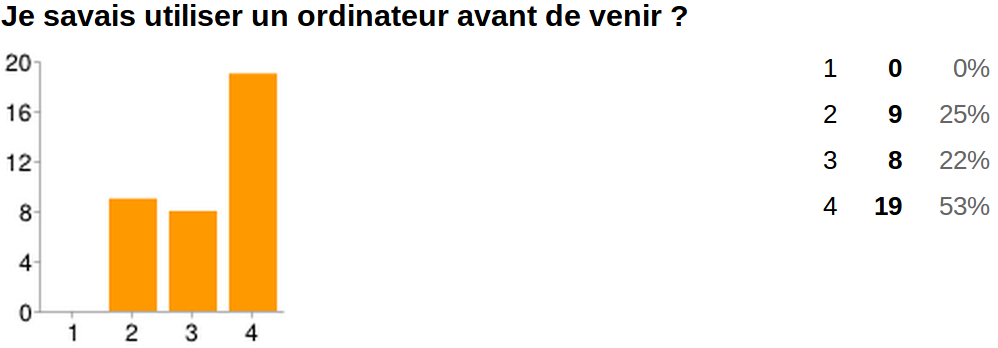
\includegraphics[scale=0.3]{content/8-validation/images/avant}
    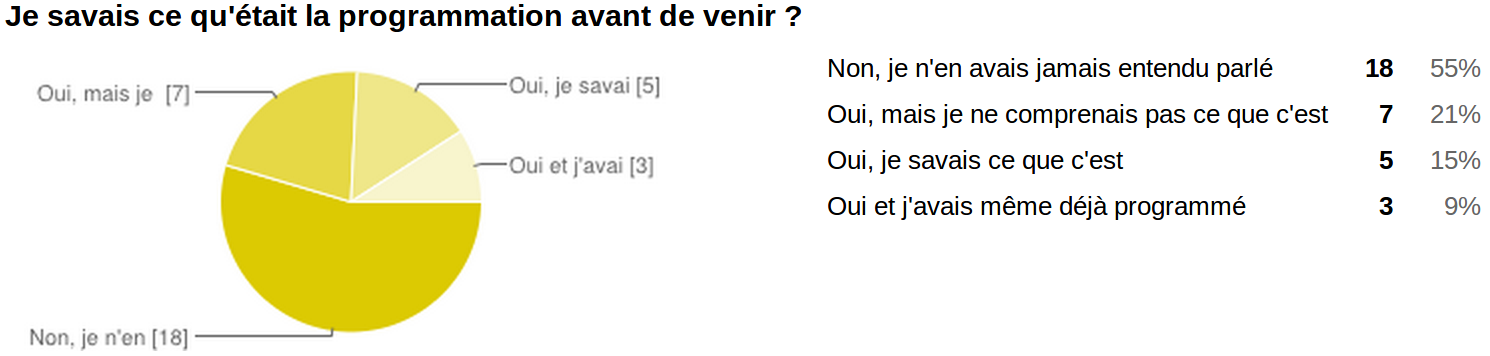
\includegraphics[scale=0.2]{content/8-validation/images/programmation}
    \caption{Auto estimation du niveau en informatique et en programmation des participants avant l'activité}
    \label{fig:niveau-avant}
  \end{center}
\end{figure}
\begin{figure}[ht]
  \begin{center}
    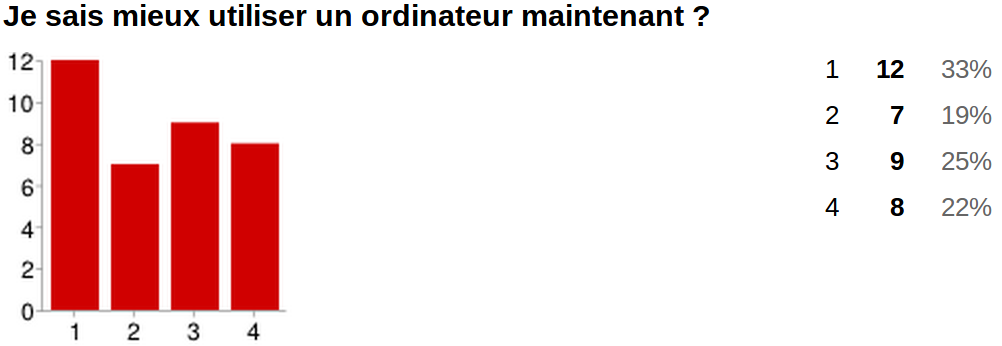
\includegraphics[scale=0.3]{content/8-validation/images/apres}
    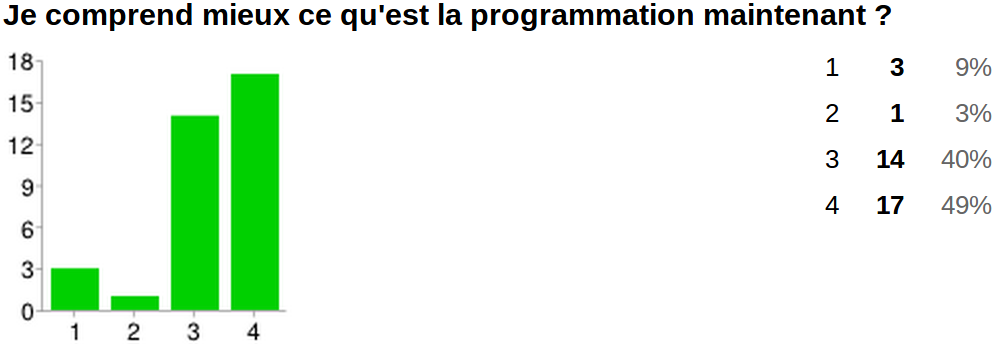
\includegraphics[scale=0.3]{content/8-validation/images/apres-programmation}
    \caption{Auto estimation du niveau en informatique et en programmation des participants après l'activité}
    \label{fig:niveau-apres}
  \end{center}
\end{figure}

Au delà de l'évaluation de leur niveau, ils ont également dû évaluer séparément chaque mission. Les graphiques représentant cette évaluation sont sur la figure \ref{fig:evaluation-mission}

\begin{figure}[ht]
  \begin{center}
    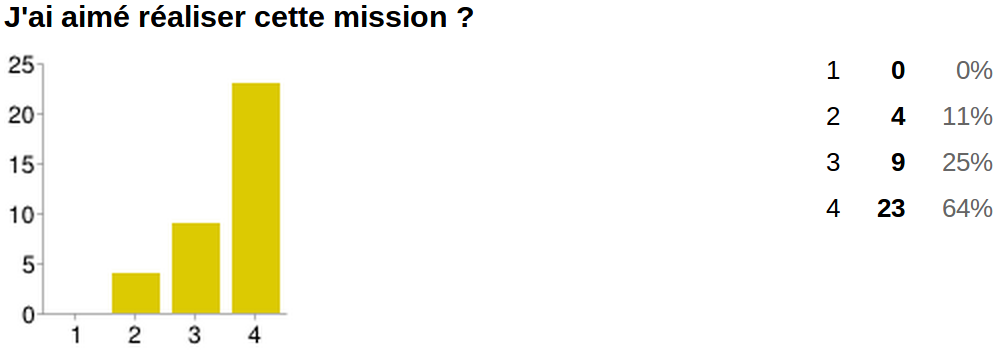
\includegraphics[scale=0.3]{content/8-validation/images/voiture}
    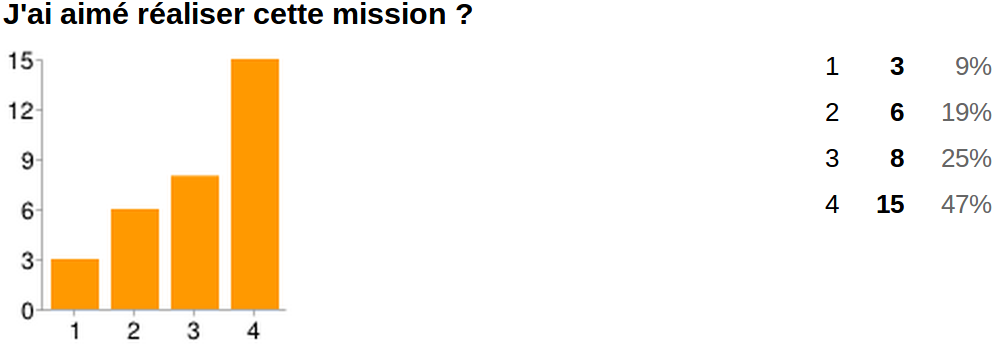
\includegraphics[scale=0.3]{content/8-validation/images/helico}
    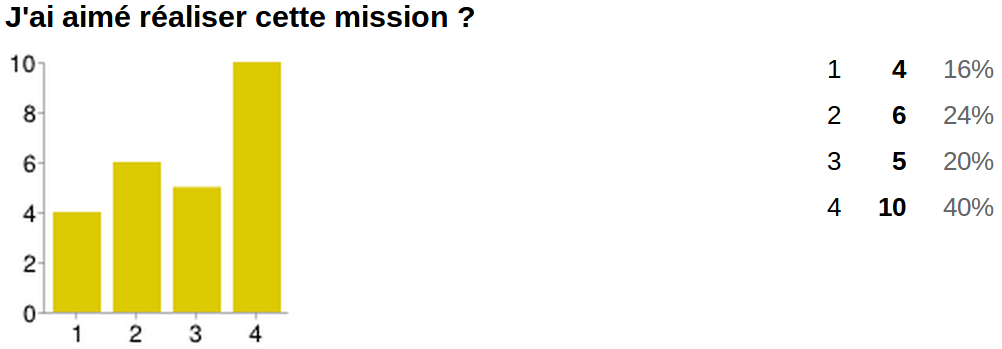
\includegraphics[scale=0.3]{content/8-validation/images/courtois}
    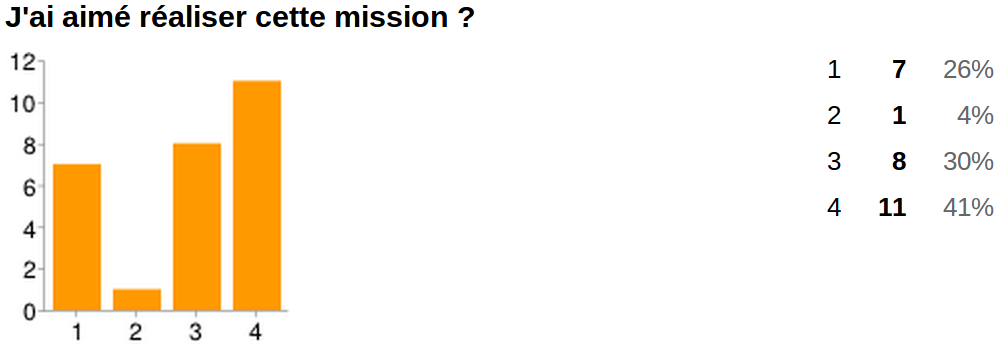
\includegraphics[scale=0.3]{content/8-validation/images/chien}
    \caption{Évaluation des missions par les enfants: En voiture \ref{mission-voiture}, hélicoptère \ref{mission-helicoptere}, soyons courtois \ref{mission-courtois}, tu ne m'attrapera jamais \ref{chien-chat}}
    \label{fig:evaluation-mission}
  \end{center}
\end{figure}


% Les grands vont plus vite

% mission voiture cool pour la structuration
% débouché sur du concret

% différence d'age
% appréciation des missions



chiffre et analyse de notre formulaire prof et student.














